\documentclass[a4paper,12pt]{report}
\usepackage[paper=a4paper]{geometry}
\usepackage{placeins}
\usepackage[warn]{mathtext}
\usepackage{graphicx}
\usepackage{amssymb}
\usepackage[justification=centering]{caption}
\usepackage[table,xcdraw]{xcolor}
\graphicspath{{C:\Users\User\Desktop\mipt\phys\lab141}}
\DeclareGraphicsExtensions{.pdf,.png,.jpg}

\usepackage[T2A]{fontenc}
\usepackage[utf8]{inputenc}
\usepackage[english,russian]{babel}
\usepackage{amsmath,amsfonts,amssymb,amsthm,mathtools}
\usepackage{wasysym}
\usepackage{wrapfig}
\author{Выполнил Мещеряков Всеволод, студент Б02-001}
\title{Отчет по лабораторной работе № 1.4.1 \\[15pt] «Изучение физического маятника»}
\date{\today}

\usepackage{ragged2e}
\justifying


\begin{document}

\maketitle

\section*{\Large Аннотация}

Работа заключается в изучении зависимости периода колебаний физического маятника от его момента инерции. Для этого используются математический маятник, секундомер, линейка, счётчик числа колебаний.

\section*{Теоретическая справка}

Движение маятника описывается уравнением:

\begin{equation}
	I \frac{d^2 \varphi}{dt^2}=M,
	\label{form1}
\end{equation}

где $I$ - момент инерции маятника, $\varphi$ - угол отклонения маятника от положения равновесия, $t$ - время, $M$ - момент сил, действующих на маятник.

В данной работе в качестве физического маятника используется стержень длиной $ l = 95.5 \pm 0.2 $ см. На нем закреплена призма, позволяющая двигать точку вращения относительно центра масс стержня. Пусть это расстояние равно $a$. Тогда по теореме Гюйгенса-Штейнера момент инерции маятника будет равен:

\begin{equation}
	I = \frac{ml^2}{12} + ma^2,
	\label{form2}
\end{equation}

где $m$ - масса маятника. Момент силы тяжести, действующий на маятник, 

\[ M = -mga \sin{\varphi}. \]

Если угол $\varphi$ мал, то 

\[ M \approx -mga\varphi. \]

Тогда

\[ ddot{\varphi} + \omega^2 \varphi = 0, \]

Где

\[ \omega^2=\frac{ga}{a^2+\frac{l^2}{12}}. \]

Решением уравнения является функция

\begin{equation}
	\varphi(t)=A\sin{\omega t + a}.
	\label{form3}
\end{equation}

В итоге период колебаний равен:

\begin{equation}
	T = \frac{2\pi}{\omega}=2\pi\sqrt{\frac{a^2+\frac{l^2}{12}}{ag}}.
	\label{form4}
\end{equation}

\subsection*{Измерения, погрешности и результат}

Определим диапазон амплитуд, в пределах которого период $T$ колебаний маятника можно считать не зависящим от амплитуды. Будем считать, что за 100 колебаний период одного почти не меняется, так как влияющая на это сила трения мала. Отклоним маятник на малый угол $\varphi_1 = 5{\circ}$, на $\varphi_2 = 10{\circ}$ и $\varphi_3 = 15{\circ}$. Результаты внесем в таблицу 1 и из нее получим периоды одного колебания для каждого из отклонений. Результаты выведем в таблицу 1.


\begin{table}[h!]
\centering
\scalebox{0.6}{
\begin{tabular}{|c|c|c|}
\hline
\cellcolor[HTML]{FFFFFF}\textbf{\begin{tabular}[c]{@{}c@{}}Угол\\       отклонения\end{tabular}} & \textbf{\begin{tabular}[c]{@{}c@{}}Время \\      100 колебаний, с\end{tabular}} & \textbf{\begin{tabular}[c]{@{}c@{}}Среднее время\\      100 колебаний, с\end{tabular}} \\ \hline
5                                                                                                & 161.04                                                                          & 161.1                                                                                  \\ \hline
10                                                                                               & 161.32                                                                          & 161.1                                                                                  \\ \hline
15                                                                                               & 160.94                                                                          & 161.1                                                                                  \\ \hline
\end{tabular}
}
\caption{\textit{Измерение зависимости периода одного колебания от угла отклонения.}}
\end{table}

Как видим из таблицы 1, период колебания не зависит от угла отклонения, если угол малый. 

\begin{table}[h!]
\centering
\scalebox{0.65}{
\begin{tabular}{|c|c|c|c|c|c|c|}
\hline
\cellcolor[HTML]{FFFFFF}\textbf{\begin{tabular}[c]{@{}c@{}}Случайная \\ погрешность\\ измерения\\ времени\\ 100 колебаний, с\end{tabular}} & \textbf{\begin{tabular}[c]{@{}c@{}}Погрешность\\ в связи\\ с реакцией\\ человека, с\end{tabular}} & \textbf{\begin{tabular}[c]{@{}c@{}}Полная\\  погрешности\\ измерения\\ времени\\ 100 колебаний, с\end{tabular}} & \textbf{\begin{tabular}[c]{@{}c@{}}Период\\ одного\\ колебания,\\ с\end{tabular}} & \textbf{\begin{tabular}[c]{@{}c@{}}Погрешности\\ измерения\\ периода\\ одного\\ колебания, с\end{tabular}} & \textbf{\begin{tabular}[c]{@{}c@{}}Средний \\ период , \\ c\end{tabular}} & \textbf{\begin{tabular}[c]{@{}c@{}}Погрешность\\ измерения\\ среднего\\ периода, с\end{tabular}} \\ \hline
0.06                                                                                                                                       & 0.2                                                                                               & 0.21                                                                                                            & 1.611                                                                             & 0.021                                                                                                      & 1.611                                                                     & 0.025                                                                                            \\ \hline
0.22                                                                                                                                       & 0.2                                                                                               & 0.30                                                                                                            & 1.611                                                                             & 0.030                                                                                                      & 1.611                                                                     & 0.025                                                                                            \\ \hline
0.16                                                                                                                                       & 0.2                                                                                               & 0.26                                                                                                            & 1.611                                                                             & 0.026                                                                                                      & 1.611                                                                     & 0.025                                                                                            \\ \hline
\end{tabular}
}
\caption{\textit{Погрешности вычисления периода колебаний.}}
\end{table}

В таблице 2 приведены погрешность определения периода колебаний $T_1$ и само его значение.

Будем перемещать призму и замерять время 100 колебаний для каждого положения крепления. Результаты отразим в таблице 3. На основании этих данных составим точки для графика зависимости $T^2a$ от $a^2$. Погрешность точек ординаты будем считать по формуле:

\[ \sigma_{T^2a}=T^2a\cdot\sqrt{4(\frac{\sigma_{T^2}}{T^2})^2+(\frac{\sigma_a}{a})^2}. \]

Погрешности $T$ и $a$ - время реакции человека и инструментальная соответственно. Погрешность $T^2$ будем считать по формуле $\sigma_{T^2}=2\sigma_T $. Вычисления и их результаты приведем в таблице 4.

\begin{table}[]
\centering
\begin{tabular}{|c|c|c|c|}
\hline
\cellcolor[HTML]{FFFFFF}\textbf{\begin{tabular}[c]{@{}c@{}}$T^2a$, \\ $м\cdot с^2$\end{tabular}} & \textbf{\begin{tabular}[c]{@{}c@{}}$a^2$, \\ $м^2$\end{tabular}} & \textbf{\begin{tabular}[c]{@{}c@{}}$\sigma_{T^2a}$,\\  $м\cdot с^2 $\end{tabular}} & \textbf{\begin{tabular}[c]{@{}c@{}}$\sigma_{a^2}$,\\ $м^2$\end{tabular}} \\ \hline
1.144                                                                                    & 0.198                                                          & 0.029                                                                      & 0.004                                                                  \\ \hline
1.051                                                                                    & 0.170                                                          & 0.027                                                                      & 0.004                                                                  \\ \hline
0.881                                                                                    & 0.127                                                          & 0.023                                                                      & 0.004                                                                  \\ \hline
0.766                                                                                    & 0.103                                                          & 0.021                                                                      & 0.004                                                                  \\ \hline
0.711                                                                                    & 0.092                                                          & 0.019                                                                      & 0.004                                                                  \\ \hline
0.595                                                                                    & 0.066                                                          & 0.017                                                                      & 0.004                                                                  \\ \hline
0.558                                                                                    & 0.055                                                          & 0.016                                                                      & 0.004                                                                  \\ \hline
0.400                                                                                    & 0.024                                                          & 0.012                                                                      & 0.004                                                                  \\ \hline
0.323                                                                                    & 0.013                                                          & 0.010                                                                      & 0.004                                                                  \\ \hline
\end{tabular}
\caption{\textit{Точки для графика зависимости $T^2a$ от $a^2$.}}
\end{table}


\begin{table}[h]
\centering
\scalebox{0.9}{
\begin{tabular}{|c|c|c|c|c|}
\hline
\cellcolor[HTML]{FFFFFF}\textbf{\begin{tabular}[c]{@{}c@{}}Расстояние\\ от центра масс\\ до точки\\ крепления, м\end{tabular}} & \textbf{\begin{tabular}[c]{@{}c@{}}Время\\ 100\\ колебаний,с\end{tabular}} & \textbf{\begin{tabular}[c]{@{}c@{}}Погрешность\\  измерения, с\end{tabular}} & \textbf{\begin{tabular}[c]{@{}c@{}}Период\\ одного, с\end{tabular}} & \textbf{\begin{tabular}[c]{@{}c@{}}Погрешность\\ определения\\ периода\\ одного, с\end{tabular}} \\ \hline
0.445                                                                                                                          & 160.32                                                                   & 0.2                                                                          & 1.60                                                                & 0.02                                                                                             \\ \hline
0.412                                                                                                                          & 159.71                                                                   & 0.2                                                                          & 1.60                                                                & 0.02                                                                                             \\ \hline
0.357                                                                                                                          & 157.08                                                                   & 0.2                                                                          & 1.57                                                                & 0.02                                                                                             \\ \hline
0.321                                                                                                                          & 154.52                                                                   & 0.2                                                                          & 1.55                                                                & 0.02                                                                                             \\ \hline
0.303                                                                                                                          & 153.16                                                                   & 0.2                                                                          & 1.53                                                                & 0.02                                                                                             \\ \hline
0.257                                                                                                                          & 152.16                                                                   & 0.2                                                                          & 1.52                                                                & 0.02                                                                                             \\ \hline
0.234                                                                                                                          & 154.41                                                                   & 0.2                                                                          & 1.54                                                                & 0.02                                                                                             \\ \hline
0.155                                                                                                                          & 160.64                                                                   & 0.2                                                                          & 1.61                                                                & 0.02                                                                                             \\ \hline
0.112                                                                                                                          & 169.7                                                                    & 0.2                                                                          & 1.70                                                                & 0.02                                                                                             \\ \hline
\end{tabular}
}
\caption{\textit{Зависимость периода от расстояния между центром масс и точкой вращения.}}
\end{table}

Построим аппроксимирующую прямую $T^2a$ от $a^2$ по методу наименьших квадратов - рисунок 2. Отсюда получаем коэффициенты наклона и смещения:

\[ k = 0.0442 [c^2/см] \]
\[ b = 29.783 [см \cdot с^2] \] 

Погрешность коэффициентов рассчитаем по формулам для МНК:

\[ \sigma_k=\sqrt{\frac{\frac{D_{xx}}{D_{yy}}-k^2}{n-2}} = 0.00486 [с^2/см], \epsilon_k \approx 11 \% \]

\[ \sigma_b=b\sqrt{<x^2>} = 3.574 [см \cdot с^2], \epsilon_b \approx 12 \% \]

Получим выражение для $T^2a$ из (4):

\[ T^2a=\frac{4\pi^2a^2}{g}+\frac{4\pi^2}{g}\cdot\frac{l^2}{12}. \]

Так как график аппроксимирующей прямой имеет вид $ y = kx + b $, то

\[ k = \frac{4\pi^2}{g}, \]
\[ b = \frac{kl^2}{12}. \]

Тогда получим значения $g$ и $l$:

\[ g = \frac{4\pi^2}{k} \pm \frac{4\pi^2}{k} \cdot \frac{\sigma_k}{k} = 8.9 \pm 0.1 [м/с^2]. \]

\[ l =  \sqrt{\frac{12b}{k}} \pm \sqrt{\frac{12b}{k}}\cdot \frac{1}{2}\sqrt{(\frac{\sigma_b}{b})^2+(\frac{\sigma_k}{k})^2} = 89.9 \pm 7 [см] \]

Теперь подберем длину математического маятника так, чтобы его период совпал с периодом физического маятника с расстоянием от оси до центра равным $a = 0.47 м $, длина физического маятника $l = 0.95 м$. Тогда его приведенная длина $l_{пр}=a+\frac{l^2}{12a} \approx 0.63 м$. Подобраянная длина же $0.64$. Как видно, длины почти что совпадают. Проверим на опыте - запишем время 100 колебаний для физического маятника с $a=0.47 м$ и математического маятника с $l=0.64 м$. Получим:

\[ T_ф = 160.42 с, T_м = 161.4 с.\]

Тогда периоды отличаются менее чем на 1 тысячную секунды. Из чего делаем вывод, что длина была подобрана верно.


\begin{figure}[h]
\center{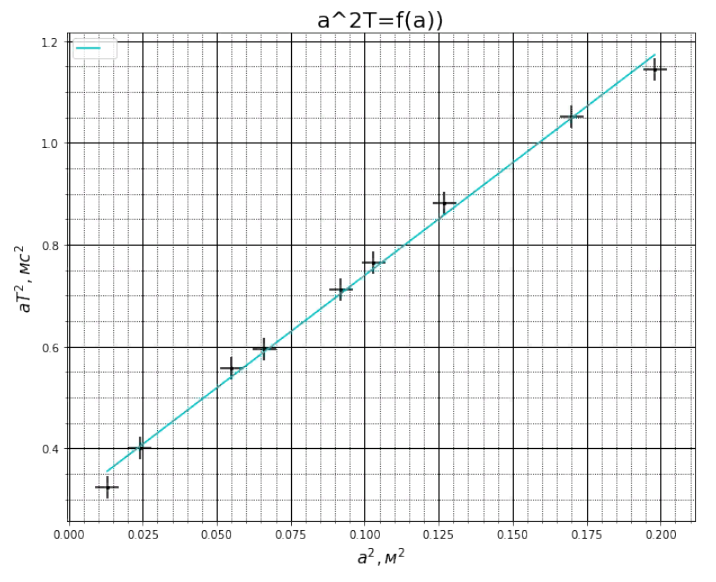
\includegraphics[scale=1]{lab141ris2.png}}
\caption{\textit{График зависимости $T^2a$ от $a^2$}}
\end{figure}


\end{document}






